\documentclass[12pt,a4paper,twoside]{book}


\usepackage[a4paper,inner=3.5cm,outer=2.5cm]{geometry}
\usepackage[titletoc,title,toc,page]{appendix}
\usepackage{verbatim}
\usepackage{placeins}
\usepackage{listings}
\usepackage[english]{babel}
\usepackage{tikz}
\usepackage{parskip}
\usepackage{graphicx}
\usepackage{blindtext}
\usepackage{chngcntr}
\usepackage{amsmath}
\usepackage{amssymb}
\counterwithin{table}{chapter}
\usepackage{newlfont}
\usepackage{fancyhdr}
\usepackage{indentfirst}
\usepackage[utf8]{inputenc}
\usepackage{float}
\usepackage{hyperref}
\usepackage[capitalize,noabbrev]{cleveref}
\usepackage{soul}
\usepackage[font=footnotesize,labelfont=bf]{caption}
\usepackage{multirow}
\usepackage{hyphenat}
\hyphenation{mate-mati-ca recu-perare}

\usepackage{lscape}
\usepackage{natbib}
\bibliographystyle{unsrt}
\setcitestyle{numbers,open={[},close={]}}

\newcommand{\rom}[1]{\uppercase\expandafter{\romannumeral #1\relax}}
\newif\ifofficial
\ifdefined\officialbuild \officialtrue \fi

\usepackage{pdfpages}

\hypersetup{
    pdftitle={Privacy-Preserving Decentralized Crowdsensing: a Smart Contract-based approach},
    pdfauthor={Daniele Romanella},
}

%lstlisting configuration
\lstset{
    backgroundcolor=\color{gray!10},    % sfondo grigio chiaro
    frame=single,                       % bordo su tutti i lati
    numbers=left,                       % numeri di riga a sinistra
    numberstyle=\tiny\color{darkgray},      % numeri piccoli e grigi
    basicstyle=\ttfamily\small,         % font monospace
    breaklines=true,
    captionpos=b
}

\lstdefinelanguage{typescript}{
    keywords={abstract, any, as, boolean, break, case, catch, class, console, const, constructor, continue, debugger, declare, default, delete, do, else, enum, export, extends, false, finally, for, from, function, get, if, implements, import, in, instanceof, interface, is, let, module, namespace, new, null, number, of, package, private, protected, public, readonly, require, return, set, static, string, super, switch, this, throw, true, try, type, typeof, var, void, while, with, yield},
    keywordstyle=\color{teal}\bfseries,
    ndkeywords={log},
    ndkeywordstyle=\color{violet}\bfseries,
    identifierstyle=\color{black},
    sensitive=true,
    comment=[l]{//},
    morecomment=[s]{/*}{*/},
    commentstyle=\color{gray}\ttfamily,
    stringstyle=\color{orange}\ttfamily,
    morestring=[b]',
    morestring=[b]"
}


\lstdefinelanguage{solidity}{
    keywords={address, anonymous, as, assembly, assert, break, calldata, case, constant, constructor, continue, contract, default, delete, do, else, emit, enum, event, fallback, false, for, from, function, if, indexed, inherit, interface, internal, is, let, library, mapping, modifier, new, payable, pragma, private, public, pure, receive, require, return, returns, revert, solidity, storage, struct, success, switch, this, throw, true, try, type, typeof, using, view, while},
    keywordstyle=\color{teal}\bfseries,
    ndkeywords={string, uint, uint256, int, bool, bytes, bytes32},
    ndkeywordstyle=\color{violet}\bfseries,
    identifierstyle=\color{black},
    sensitive=true,
    comment=[l]{//},
    morecomment=[s]{/*}{*/},
    commentstyle=\color{gray}\ttfamily,
    stringstyle=\color{orange}\ttfamily,
    morestring=[b]"
}

\begin{document}
% Per spostare i vari elementi più su o più giù gioca con i valori di vspace che ci sono tra uno e l'altro
    \pagestyle{empty}
    \newgeometry{
    left=20mm,
    right=20mm,
    top=20mm,
    bottom=20mm
}
\begin{titlepage}

    \begin{center}

        
\includegraphics[width=6.5cm,height=4.7cm]{img/marchio-di-ateneo}

        \vspace{10mm}

        {\large{\bf{Dipartimento di Informatica - Scienza e ingegneria}}}

        \vspace{5mm}

        {\Large{\bf{Corso di Laurea magistrale in Informatica}}}

        \vspace{15mm}

        {\Huge{\bf Titolo della tesi }}\\
        \vspace{3mm}
        {\Huge{\bf anche su più}}\\
        \vspace{3mm}
        {\Huge{\bf righe }}\\
        \vspace{3mm}

    \end{center}

    \vspace{10mm}

    \begin{minipage}[t]{0.40\textwidth}
    {\Large{\bf Relatore: \\ Chiar.mo Prof.\\ Stefano Ferretti}}

        \vspace{3mm}

        {\Large{\bf Correlatore: \\ Chiar.mo Prof.\\ Luca Bedogni}}
    \end{minipage}
    \hfill
    \begin{minipage}[t]{0.40\textwidth}\raggedleft
    {\Large{\bf Presentata da: \\ Daniele Romanella}}
    \end{minipage}

    \vspace{30mm}

    \rule[0.5cm]{15.8cm}{0.6mm}

    \begin{center}
    {\large{\bf I sessione \\}}
    {\large{\bf Anno Accademico 2025/2026\\}}
    \end{center}

\end{titlepage}
\restoregeometry
    \newpage~\newpage
    \ifofficial\else
        \topmargin=6.5cm
\begin{flushright}
    \emph{
        \LARGE{Troverò una strada, o ne costruirò una.}\\\vspace{2mm}
    }
\end{flushright}

\pagenumbering{gobble}
        \newpage~\newpage
    \fi
    \topmargin=-1cm
\chapter*{Sommario}
Il crowdsensing mobile consente la raccolta distribuita di dati
geografici aggregando i contributi di un elevato numero di
partecipanti.
Questo paradigma si presta a scenari eterogenei come ad esempio: monitoraggio
ambientale, analisi del traffico urbano, raccolta di dati
epidemiologici.
Scenari in cui la granularità spaziale e la scalabilità
del numero di contributori sono requisiti primari.


Le soluzioni esistenti affidano il coordinamento della campagna a
un server centralizzato, introducendo un unico punto di fiducia
che può compromettere la riservatezza dei dati raccolti e la
privacy dei partecipanti.
Un server centralizzato può essere compromesso, può colludere con
terze parti o essere soggetto a guasti, rendendo fragile l'intero
sistema.

Questa tesi presenta il design, l'implementazione e la valutazione
di un protocollo di crowdsensing decentralizzato e rispettoso della
privacy, in cui il coordinamento è delegato a uno smart contract
Ethereum.


Lo smart contract sostituisce il server fidato con un intermediario
pubblicamente verificabile e resistente alle manomissioni: la sua
logica è eseguita deterministicamente dall'Ethereum Virtual
Machine (EVM), ogni nodo della rete ne mantiene una copia, e il
comportamento del contratto non può essere alterato da alcuna
singola parte dopo il deploy.

Il protocollo coinvolge tre attori principali.
Il campaign initiator, \texttt{B} avvia la campagna, definisce i parametri
spaziali e distribuisce le chiavi crittografiche.
I sender raccolgono e inviano i dati geografici.
I verifier, selezionati casualmente dal contratto, validano le
submission esprimendo un voto di approvazione o rifiuto.
La partecipazione di sender e verifier è regolata da un meccanismo
di cauzione tramite token ERC-20 personalizzato, \texttt{DST}: il deposito
viene restituito al termine della campagna, unitamente al reward,
solo ai partecipanti onesti.

La riservatezza dei dati è garantita attraverso crittografia
ibrida.
Ogni sender cifra il proprio payload con una chiave simmetrica
AES-256-GCM e cifra quest'ultima con la chiave pubblica RSA del
verifier eletto tramite RSA-OAEP.
Il testo cifrato viene archiviato off-chain su IPFS; on-chain viene
pubblicato esclusivamente il Content Identifier~(CID) cifrato.

L'area della campagna è suddivisa in una griglia spaziale di chunk:
il contratto valida on-chain l'origine geografica di ciascuna
submission e limita il numero di dati accettati per chunk,
prevenendo la sovra-rappresentazione delle zone ad alta densità di
partecipanti.

Un'analisi di sicurezza e incentivi del protocollo base individua
tre problemi aperti.
Primo, un verifier malevolo può accedere ai dati in chiaro prima di
esprimere il proprio verdetto, falsando la valutazione.
Secondo, la distribuzione geografica dei reward non incentiva i
sender a contribuire alle aree meno coperte, favorendo la
concentrazione nelle zone già sature.
Terzo, i verifier che esprimono voti errati non subiscono alcuna
conseguenza economica, oltre alla perdita del deposito cauzionale,
rendendo conveniente il comportamento scorretto.
La correttezza del protocollo base rispetto agli obiettivi di
segretezza e autenticazione è verificata formalmente con ProVerif
sotto il modello di attaccante Dolev-Yao, solo nel caso in cui gli attori si comportino onestamente e nel caso in cui l'avversario $\mathcal{A}$ non si autentichi come verifier.

Un secondo contratto Solidity, \texttt{PSC}, estende il protocollo base
affrontando ciascuno dei tre problemi.
Per il problema del verifier malevolo, PSC introduce un ulteriore
strato crittografico: \texttt{B}, per ogni dato inviato crea una coppia di chiavi asimmetriche.
Quindi \texttt{B} decifra il dato inviato, riesegue l'upload del dato cifrato su IPFS e successivamente attraverso la chiave pubblica dei verificatori eletti distribuisce la chiave di decrittazione del dato da verificare.

Per lo squilibrio geografico dei reward, PSC implementa una funzione
di decadimento basata sul rapporto di saturazione del chunk: il
reward per una submission verso un chunk già parzialmente saturo
viene ridotto secondo la formula~$(1 - \alpha)^{1/2^k}$, dove
$\alpha$~è il rapporto di saturazione e~$k$~è un parametro
configurabile che controlla la ripidità del decadimento.

La radice frazionaria viene calcolata on-chain tramite il metodo
babilonese iterativo, evitando operazioni in virgola mobile non
supportate dall'EVM.

Per l'assenza di penalità, PSC traccia i voti corretti e scorretti
di ciascun verifier e consente al campaign initiator di espellere
i verifier che superano una soglia configurabile di voti errati.

L'implementazione comprende i due contratti Solidity documentati,
un SDK TypeScript che espone un'API per-attore e gestisce le
operazioni crittografiche off-chain, e una suite di test completa
sviluppata con Hardhat.

Le ottimizzazioni di gas documentate includono la gestione della
pending list tramite swap-and-pop al posto dello shift lineare FIFO,
la compressione delle struct in un singolo slot EVM da 32~byte,
l'aritmetica \texttt{unchecked} nelle funzioni di reward, e
l'eliminazione dei dati di enrollment tramite \texttt{delete} dopo
il loro utilizzo.

La valutazione empirica copre tre dimensioni.
L'analisi dei costi di gas su 16~scenari, con sender e verifier
nell'intervallo~$\{1, 10, 100, 1000\}$, mostra che il contratto
ottimizzato riduce i costi del verifier del~98\% rispetto alla
baseline FIFO.
La baseline FIFO risulta non praticabile su reti Fusaka-era in tutti
i 16~scenari, superando il limite per-transazione di~$2^{24}$~gas
introdotto dall'EIP-7825 di un fattore~$3.4\times$.
PSC aggiunge un overhead contenuto rispetto a PFC, con l'incremento
più significativo sulla data submission dovuto al calcolo del reward decaduto.

Su reti L2 quali Arbitrum e Optimism, il costo di partecipazione
diventa trascurabile per tutti i ruoli.
L'analisi della saturazione dei blocchi sotto campagne concorrenti
evidenzia una sezione critica sulla capacità del blocco: con quattro
campagne parallele, il numero medio di blocchi consumati per
campagna raggiunge~$3.65\times$.
La simulazione spaziale sul dataset di traiettorie taxi della città
di Porto valida il meccanismo di decadimento del reward, mostrando
come la funzione redistribuisca efficacemente gli incentivi verso le
aree meno coperte.
La copertura geografica satura attorno al~50\% tra 500 e
1\,000~sender, un limite attribuibile alla concentrazione geografica
delle traiettorie nell'area urbana centrale piuttosto che al
protocollo.

I risultati confermano la fattibilità del protocollo su reti L2
e su blockchain a basso costo del gas.
Le direzioni future includono l'eliminazione del trust residuo nel
campaign initiator tramite Proxy Re-Encryption decentralizzata,
l'estensione della verifica formale a scenari di enrollment
disonesto, e la validazione su dataset con distribuzione geografica
più uniforme.
    \newpage~\newpage
    \chapter*{Abstract}
Mobile crowdsensing enables the collection of distributed geographic data
by aggregating contributions from a large number of participants, each
equipped with a sensing device.
Existing solutions rely on a centralised server to coordinate the campaign,
introducing a single point of trust that can compromise data confidentiality
and participant privacy.

This thesis presents a privacy-preserving decentralised crowdsensing protocol
in which coordination is delegated to an Ethereum smart contract, replacing
the trusted server with a publicly verifiable and tamper-resistant intermediary.
Data confidentiality is achieved through hybrid encryption: each sender
encrypts their payload with a symmetric key distributed by the campaign
initiator, and stores the ciphertext on IPFS, publishing only the encrypted
content identifier on-chain.
Participation is incentivised through a custom ERC-20 token and a bond
mechanism, while the campaign area is partitioned into a spatial grid of
chunks to validate the geographic origin of each submission and prevent
over-representation of densely populated areas.
A second contract extends the base protocol by addressing three open issues:
verifier access to plaintext data before verdict, lack of geographic reward
incentives, and absence of penalties for incorrect votes.

An empirical evaluation covers gas consumption across multiple networks,
block capacity contention under concurrent campaign execution, and spatial
coverage on a real-world taxi trajectory dataset from the city of Porto.
The results show that the optimised contract reduces verifier gas costs by
approximately $98\%$ relative to the FIFO baseline, and that the reward
decay mechanism successfully redirects sender contributions towards
underrepresented areas.
On some Layer 2 networks, the cost of participation becomes negligible for all
roles.

\topmargin=-1cm
    \newpage~\newpage
    \tableofcontents
\thispagestyle{empty}
\listoftables
\thispagestyle{empty}
\listoffigures
\thispagestyle{empty}
\lstlistoflistings
\thispagestyle{empty}
    \newpage~\newpage

    % settings
    \pagenumbering{arabic}
    \setcounter{chapter}{-1}
    \raggedbottom


    % thesis starts here
    \chapter{Introduction} \label{ch:intro}
\pagestyle{plain}
\setcounter{page}{1}
    \chapter{Background} \label{ch:background}
This chapter introduces all the background concepts required to understand the protocol and the context in which it works.
\section{Network architectures} \label{sec:network-architectures}
Network architecture defines how nodes communicate and interact over a network.
The most common architectural models are introduced in the following subsections.
\subsection{Distributed systems} \label{subsec:distributed-systems}
A distributed system is a collection of independent nodes that communicate and coordinate over a network to appear as a single coherent system~\cite{van2002distributed}.
This model enables horizontal scaling and eliminates single points of failure, making it suitable for high availability applications.
\subsection{Client-Server} \label{subsec:client-server}
The client-server architecture is one of the most widely adopted
architectural models~\cite{van2002distributed}.
It involves two types of nodes:
\begin{itemize}
    \item \textbf{Server}: the node responsible for delivering content
    and services to clients, maintained by the service provider.
    \item \textbf{Client}: the node that communicates with the server
    to request a specific service or resource.
\end{itemize}
These two node types communicate with each other following a
request-response model, where the client initiates the interaction
and the server responds accordingly.
\newline
Some protocols based on Client-Server architectures are:
\begin{itemize}
    \item \textbf{HTTP}: Client sends an HTTP request and receives an HTTP Response~\cite{rfc9110}
    \item \textbf{DNS}: Client (Resolver) sends a DNS query to DNS server to resolve a name~\cite{rfc1034}
    \item \textbf{DHCP}: Client broadcasts a DHCP request over all the local network and if a DHCP server is listening it will handle the IP assignation~\cite{rfc2131}
\end{itemize}

\subsection{Peer-to-peer} \label{subsec:peer-to-peer}
Peer-to-peer architectures are adopted in contexts where a single server is not able to guarantee a service, where the decentralization is a required property for the model or where the goal is to remove a single point of failure.~\cite{van2002distributed}

In a peer-to-peer context all nodes act as both client and server, simultaneously.
Each node is called \texttt{peer}, and it is able to request and provide resources to other peers.

In peer-to-peer protocols there is a challenge: peer discovery,
the mechanism by which a node locates other peers to communicate with.
A common approach is centralized trackers, where a server maintains a list
of active peers, but this reintroduces a single point of failure.
Distributed hash tables (DHT) solve this by distributing peer information
across the network itself, removing any central dependency~\cite{maymounkov2002kademlia}.

An example of a peer-to-peer protocol is BitTorrent~\cite{cohen2003incentives}, widely used for distributed file sharing.
The peer-to-peer model also serves as the foundation for distributed storage systems such as IPFS, discussed
in the following subsection.
\subsection{IPFS} \label{subsec:ipfs}
IPFS (InterPlanetary File System) is a peer-to-peer distributed file system that enables efficient and reliable data distribution among all nodes~\cite{benet2014ipfs}.
Unlike traditional location based addressing, each piece of content is identified by its cryptographic hash, known as a Content Identifier (CID).
The protocol works in the following way: every node hosts and shares a portion of the data, when a client requests a specific CID, it uses the DHT to retrieve the data from the nodes that store it.
In addition, IPFS is a versioned file system and it supports integration with decentralized applications, offering a storage layer for blockchains and Web3 ecosystems.
\section{Blockchain}\label{sec:blockchain}
A blockchain is a growing distributed ledger that stores data in an ordered sequence of blocks~\cite{bitcoin}.
Each block contains a set of transactions, the hash of the previous block, and a timestamp; this structure creates a chain.
This chained structure makes the blockchain transactions resistant to alteration, because, when the transactions are registered,
an adversary $\mathcal{A}$ would need to produce a block with the same hash, which is infeasible in probabilistic polynomial time~\cite{bitcoin}.
\subsection{Ethereum}\label{subsec:eth}
\subsection{Smart Contract}\label{subsec:sc}
\subsection{Gas}\label{subsec:gas}
\section{Crowdsensing}\label{sec:crowdsensing}
\section{Related work and state of the art} \label{sec:related-work}
    \chapter{Protocol design} \label{ch:protocol-design}
In this chapter the protocol design is presented.
The protocol leverages smart contracts and asymmetric encryption to ensure confidentiality and data integrity.
The protocol adopts a multi-layered encryption approach, performed off-chain, and uses the smart contract as a communication channel for the crowdsensing campaign.
The key exchange is made to and from the campaign initiator (referred from now as \"\texttt{B}\").
\texttt{B} uses their private/public key pair for enhancing confidentiality, in this way, only \texttt{B} can access the other actors' public key, namely senders (\texttt{S}) and verifiers (\texttt{V}).
This approach shares similarities with prior work on asymmetric key exchange mediated by smart contracts~\cite{muth2020smartdhx}, although it differs substantially in both application domain and protocol design.

\section{Actors}\label{sec:actors}
The protocol involves several actors that are described in the following subsections.
\subsection{Campaign initiator}\label{subsec:campaign-initiator}
The campaign initiator (\texttt{B}) is the actor interested for collecting data for some reason.
They define the geographic area where the smart contract works and set the smart contract hyperparameters, all configurable parameters are explained in Appendix~\ref{ch:appendix-a-parameters}.
In addition they deposit the reward funds into the smart contract to ensure that funds are available and senders and verifiers can be compensated.
The details of rewarding model are described in the~\ref{subsec:proto-rewarding-model} subsection.

\subsection{Sender}\label{subsec:sender}
\subsection{Verifier}\label{subsec:verifiers}

\section{Protocol workflow}\label{sec:proto-workflow}
\subsection{Initialization}\label{subsec:proto-init}
\subsection{Enrollment}\label{subsec:proto-enrollment}
\subsection{Data submission}\label{subsec:proto-datasubmit}
\subsection{Verification}\label{subsec:proto-verification}
\subsection{Data publishing}\label{subsec:proto-data-publish}
\subsection{Rewarding model}\label{subsec:proto-rewarding-model}
\subsection{Bond model}\label{subsec:proto-bond-model}
\section{Security analysis and issues}\label{sec:security-analysis-issues}
    \chapter{Smart contract implementation}\label{ch:implementation}
In the previous chapter the protocol was explained, some issues are identified, and mitigation strategies are proposed for the most critical ones.
This chapter describes how the entire protocol is implemented.
The development environment is made of Solidity on Ethereum~\cite{ethereum} and Hardhat as the development and testing framework.
In addition, the chapter also describes how \texttt{PrivacyFirstContract} and its extension, \texttt{PrivacySecondContract} interacts and which functions are overridden and the motivation behind every choice.

\section{Architecture}\label{sec:implementation-architecture}
The architecture is divided between on-chain operations and off chain ones, this distinction exists
because a lot of actions are not executable on the blockchain, like IPFS upload/download and ciphers
usage are not permitted on smart contacts due to the non-deterministic nature of operations such as encryption~\cite{wood2014ethereum}.
The off-chain operations are encapsulated in a SDK that allows actors to interact with the protocol without dealing directly with blockchain primitives.
The structure is composed by two contracts: the base protocol inspired to~\cite{bedogni2024crowdsensing} and another one that extends the base protocol with the mechanisms proposed in Section~\ref{sec:addressing-issues}.

\subsection{Contract hierarchy}\label{subsec:implementation-contract-hierarchy}
The \texttt{PrivacySecondContract} extends \texttt{PrivacyFirstContract}, reusing its core logic without modification.
The functionalities not covered by Section~\ref{sec:addressing-issues}, such as sender enrollment, bond system, majority consensus, and lifecycle are inherited without modification.
An overview of functions and more representative fields are shown in Figure~\ref{fig:proto-implementation-contract-hierarchy}.
\begin{figure}
    \begin{center}
        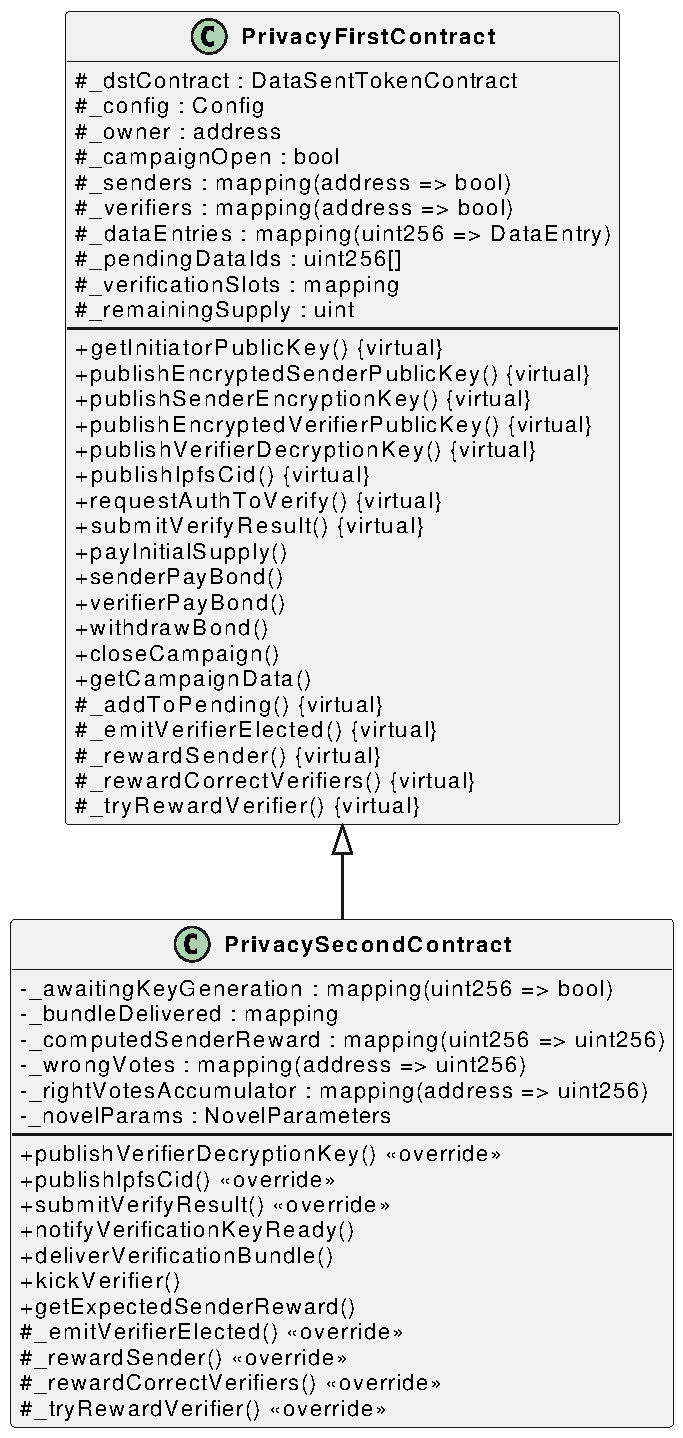
\includegraphics[width=0.50\textwidth]{diagrams/proto-implementation-contract-hierarchy-out}
        \caption{Class hierarchy of the two smart contracts}\label{fig:proto-implementation-contract-hierarchy}
    \end{center}\label{fig:proto-implementation-contract-hierarchy-container}
\end{figure}

There are four \texttt{internal} functions that have been overridden in the \texttt{PrivacySecondContract} to adapt them to the contract needs.

Since the extended contract needs to delivery verification bundles, to prevent duplicate delivery, a \texttt{\_bundleDelivered} mapping is introduced.
For this reason, once the bundle is sent the function \texttt{\_emitVerifierElected} is overridden in \texttt{PrivacySecondContract} to reset the delivery state, allowing a new bundle to be delivered if the verifier slot is reassigned.
This allows the usage of the same location of memory, the delivery of verification bundles is required in order to address the issue of verifiers trust, described in Section~\ref{subsec:addressing-issues-trusted-verifier-issue}.

Since in the Section~\ref{subsec:addressing-issues-geographical-incentive-issue} is described a mechanism to incentive data sensing in heterogeneous geographical areas, it is necessary to change the rewarding system.
For this reason, the method \texttt{\_rewardSender} is overridden and the only modification made is change the calculation of total payout.
In the first version of the contract, the reward is always the full base payout, in the novel one, the contract reads the pre-computed reward from storage.
The effective payout is calculated at the CID publish time, the contract execute the calculus in the \texttt{\_computeDecayedReward} function.
That function executes $k$ times the sqrt of a value (as shown in equation~\ref{eq:proto-design-reward-determination}), in \textit{O(log n)} time using the babylonian method~\cite{kosheleva2009babylonian}, to execute this operation, all values are scaled by a factor of \texttt{1E18} since the EVM, as noted in Section~\ref{sec:chunking-system}, is unable to execute floating point calculus.

The problem of missing verifiers penalties, in addition to bond loss, is discussed in Section~\ref{subsec:addressing-issues-missing-verifier-penalties}.
To address this issue, is required to modify how the smart contract collects the verifiers responses.
For this reason, the functions \texttt{\_rewardCorrectVerifiers} and \texttt{\_tryRewardVerifier} are modified and the responses are saved in mappings that keeps the count of correct votes and wrong ones.
These mappings are required to enforce the kick of systematically wrong voters, as proposed in Section~\ref{subsec:addressing-issues-missing-verifier-penalties}.

The \texttt{PrivacySecondContract} overrides also public functions; the function used to publish decryption key (\texttt{publishVerifierDecryptionKey}) in the \texttt{PrivacyFirstContract} publishes the decryption key through the VerifierEnrolled event, using a key shared among all enrolled verifiers.
In the novel contract, the function is overridden and publish the same event without the key, because, in order to avoid a single decryption key shared among all the verifiers, like described in~\ref{subsec:addressing-issues-trusted-verifier-issue}.
For these reasons, the function \texttt{publishIpfsCid}, is overridden and instead of adding the data in the pending data structure, the data entry requires that \texttt{B} to generate a per-data key pair ($KD_{enc}$, $KD_{dec}$), after which, \texttt{B} calls \texttt{notifyVerificationKeyReady} and the smart contract adds the data to pending data structure.
The novel event \texttt{VerifierElectedForData} notifies \texttt{B} that a verifier has been elected, upon which \texttt{B} delivers a verification bundle via \texttt{deliverVerificationBundle}.
Then a \texttt{VerifierVerificationBundleReady} is emitted and the verifier can finally calculate and submit the verification result using \texttt{submitVerifyResult} overridden function that checks the verification bundle delivery.

In addition, two new functions are introduced: \texttt{getExpectedSenderReward} and \texttt{kickVerifier}, the first one is informative and useful for users to understand which payout they will receive if they send data for a specific chunk in that moment.
The second one can be used from by campaign initiator \texttt{B} to exclude a verifier from the crowdsensing campaign.
In this case the verifier's bond is returned, as the exclusion from the campaign already constitutes a sufficient penalty, consistently with the design choice described in Section~\ref{subsec:addressing-issues-missing-verifier-penalties}.

A description of all overridden functions between the contracts is shown in Table~\ref{tab:contract-implementation-hierarchy-overrides}

\begin{table}
    \centering
    \begin{tabular}{|p{4cm}|p{3.5cm}|p{3.5cm}|p{2.5cm}|}
        \hline
        \textbf{Function} & \textbf{PFC} & \textbf{PSC} & \textbf{Reason} \\
        \hline
        {\texttt{publishVerifier-\newline DecryptionKey}}
        & Publishes decryption key on-chain via \texttt{VerifierEnrolled}
        & Emits \texttt{VerifierEnrolled} without key; key is generated off-chain
        & Trusted verifier flow (\ref{subsec:addressing-issues-trusted-verifier-issue}) \\
        \hline
        \texttt{publishIpfsCid}
        & Adds data to pending; reward is fixed base payout
        & Stores data awaiting key generation; computes decayed reward
        & Trusted verifier flow and reward decay (\ref{subsec:addressing-issues-trusted-verifier-issue},~\ref{subsec:addressing-issues-geographical-incentive-issue}) \\
        \hline
        \texttt{submitVerifyResult}
        & No prerequisite on bundle delivery
        & Requires \texttt{deliver-\newline Verification-\newline Bundle} to be called first
        & Trusted verifier flow (\ref{subsec:addressing-issues-trusted-verifier-issue}) \\
        \hline
        \texttt{\_emitVerifier-\newline Elected}
        & Emits election event and assigns slot
        & Additionally resets \texttt{\_bundle-\newline Delivered} flag
        & Allows bundle re-delivery on slot reassignment \\
        \hline
        \texttt{\_rewardSender}
        & Pays fixed base payout
        & Reads pre-computed reward from \newline \texttt{\_computedSender-\newline Reward}
        & Reward decay (\ref{subsec:addressing-issues-geographical-incentive-issue}) \\
        \hline
        \texttt{\_rewardCorrect-\newline Verifiers} \newline \texttt{\_tryRewardVerifier}
        & Distributes rewards based on majority
        & Additionally records correct and wrong votes per verifier
        & Verifier penalties (\ref{subsec:addressing-issues-missing-verifier-penalties}) \\
        \hline
    \end{tabular}
    \caption{Overridden functions between \texttt{PrivacyFirstContract} (PFC) and \texttt{PrivacySecondContract} (PSC)}
    \label{tab:contract-implementation-hierarchy-overrides}
\end{table}


\subsection{SDK layer}\label{subsec:implementation-sdk-layer}
TO BE EVALUATED
\section{Protocol phases implementation}\label{sec:implementation-protocol-phases}
\subsection{Initialization and deployment}\label{subsec:implementation-protocol-init}
\subsection{Sender enrollment}\label{subsec:implementation-sender-enrollment}
\subsection{Verifier enrollment}\label{subsec:implementation-verifier-enrollment}
\subsection{Data submission}\label{subsec:implementation-data-submission}
\subsection{Verification workflow}\label{subsec:implementation-verification}
\subsection{Extended protocol}\label{subsec:implementation-extended-protocol}
\section{Economic model}\label{sec:implementation-economic-model}
\subsection{DST token integration}\label{subsec:implementation-dst-integration}
\subsection{Reward logic}\label{subsec:implementation-reward}
\subsection{Bond logic}\label{subsec:implementation-bond}
\section{Gas optimization}\label{sec:implementation-gas-optimization}
\section{Contract lifecycle and state transitions}\label{sec:implementation-lifecycle}
TO BE EVALUATED
    \chapter{Evaluation}\label{ch:evaluation}
\section{Simulation setup}\label{sec:simulation-setup}
\section{Spatial simulation}\label{sec:spatial-simulation}
\section{Gas cost analysis}\label{sec:gas-analysis}
\section{Result and discussion}\label{sec:result-discussion}


    \chapter{Conclusions}\label{ch:conclusions}
This thesis presented the design, implementation, and evaluation of a
privacy-preserving decentralised crowdsensing protocol based on smart contracts.
This chapter summarizes the contributions of the work, discusses its
limitations, and outlines directions for future research.

\section{Summary of contributions}\label{sec:conclusion-contributions-summary}
The work presented in this thesis covers three main areas: protocol design,
implementation, and evaluation.

In the design phase, \texttt{PrivacyFirstContract} was developed, building
on the crowdsensing protocol proposed by Bedogni and Ferretti~\cite{bedogni2024crowdsensing}.
A subsequent security and incentive analysis identified several open issues,
which were addressed in \texttt{\seqsplit{PrivacySecondContract}}, an extension that
introduces a geographical reward decay, and a verifier penalty system.

The implementation phase produced two Solidity smart contracts reflecting
the above design, together with a TypeScript SDK layer that exposes a
per-actor API and handles off-chain cryptographic operations, providing a
complete reference implementation of the protocol.

The evaluation phase assessed the contracts along three axes: gas
consumption and its real-world cost across multiple networks, block
capacity contention under concurrent campaign execution, and spatial
coverage and reward distribution on a real-world taxi trajectory dataset
from the city of Porto.

\section{Limitations}\label{sec:conclusion-limitations}
The work presented in this thesis has several limitations.

The geographic simulation was conducted with at most 1\,000 senders due to
RAM constraints on the test machine; a larger population could not be
evaluated without dedicated infrastructure.
Furthermore, the contracts were tested exclusively on a local Hardhat node
and were not deployed on Ethereum mainnet or any L2 network, so the
gas cost figures reported in Section~\ref{sec:gas-analysis} are based on
local measurements rather than live network conditions.

At the protocol level, the centrality of the campaign initiator \texttt{B} remains
an open issue: \texttt{PrivacySecondContract} does not eliminate \texttt{B} as a
trust point, as discussed in Section~\ref{sec:security-analysis-issues}.

Finally, the ProVerif analysis described in Section~\ref{subsec:security-analysis-issues-proverif} assumes
honest enrollment: the sender and verifier enrollment channels are modelled
as private, so the attacker cannot enrol as a malicious participant.
As a consequence, the formal verification only guarantees secrecy properties
under this assumption; scenarios involving a compromised sender or verifier
are outside the scope of the model, as noted in Appendix~\ref{ch:appendix-b-proverif-v1-honest}.

\section{Future work}\label{sec:conclusion-future-work}

Several directions are open for future investigation.
The centrality of the campaign initiator \texttt{B} could be eliminated by replacing
the current key distribution mechanism with Proxy Re-Encryption(PRE)~\cite{ateniese2006pre}: senders
would encrypt their data under their own public key, and a decentralised proxy
network, such as the Threshold Network\cite{thresholdnetwork}, would re-encrypt each ciphertext
for the elected verifier without ever learning the plaintext, removing \texttt{B} as
an online trust point entirely.

The formal security analysis could be strengthened by extending the ProVerif
model to cover dishonest enrollment scenarios, or by porting the verification
to CryptoVerif~\cite{blanchet2008cryptoverif}, which operates in the computational model and provides
guarantees over concrete cryptographic primitives rather than perfect symbolic
abstractions.

On the evaluation side, the geographic simulation should be replicated on
datasets with a more uniform spatial distribution, such as rural or
multi-city traces, to assess the effectiveness of the reward decay mechanism
beyond the concentrated urban setting of the Porto taxi fleet.
Finally, the contracts should be deployed on a public testnet and subsequently
on an L2 network to validate the gas cost figures reported in
Section~\ref{sec:gas-analysis} under real network conditions and to measure
end-to-end latency across all protocol phases.
    %thesis ends here

    \bibliography{refs}
    \renewcommand{\bibsection}{}
    \newpage~\newpage
    \renewcommand{\appendixtocname}{Appendices}
\renewcommand{\appendixpagename}{Appendices}
% \pagenumbering{gobble} we want to continue numeration
\begin{appendices}
    \chapter{Smart Contract Configuration Parameters}\label{ch:appendix-a-parameters}
This appendix provides a comprehensive reference for all configurable parameters accepted by the smart contract at deployment time.
The constructor receives a
    \texttt{Config} struct, which is composed of four sub-structures:
        \texttt{SmartContractNeeds},
        \texttt{ChunkConfig},
        \texttt{RewardConfig} and \texttt{GlobalPosition}.
Each sub-structure is documented in a dedicated table below.
In addition, the constructor receives the \texttt{B} public key and the address of \texttt{DataSentTokenContract} which is the token introduced for senders and verifiers rewarding.
The details of rewarding model are described in the~\ref{subsec:proto-rewarding-model} subsection.

A convention adopted throughout the configuration is the \textbf{zero-means-unlimited} semantics: when a parameter that governs a limit is set to zero, the corresponding constraint is not enforced.
This convention is explicitly noted for each applicable parameter.

% SmartContractNeeds
\section{Campaign Requirements (\texttt{SmartContractNeeds})}\label{sec:appendix-a-needs}
The \texttt{SmartContractNeeds} structure defines the operational rules of the crowdsensing campaign, including participation limits, and data acceptance criteria.
\ref{tab:params-needs} lists each parameter with its type, constraints, and description.
\begin{table}
    \centering
    \caption{Parameters of the \texttt{SmartContractNeeds} structure.}
    \label{tab:params-needs}
    \small
    \begin{tabular}{p{3.8cm} l p{1.8cm} p{5.8cm}}
        \hline
        \textbf{Parameter} & \textbf{Type} & \textbf{Constraint} & \textbf{Description} \\
        \hline
        %\texttt{freshnessPeriod}
        %& \texttt{uint256}
        %& $\geq 0$ (0 = disabled)
        %& Reserved for future use. Intended to define a time window for data freshness validation. Currently not enforced by the contract logic. \\[6pt]
        \texttt{dataNeeded}
        & \texttt{uint256}
        & $\geq 0$ (0 = unlimited)
        & Number of positively verified data entries required to automatically close the campaign.
        When set to zero, the campaign does not auto-close based on data count alone. \\[6pt]

        \texttt{maximumDataPerChunk}
        & \texttt{uint256}
        & $\geq 0$ (0 = unlimited)
        & Maximum number of data submissions accepted within a single spatial chunk.
        Prevents over-representation of a geographic area. \\[6pt]

        \texttt{checksRequired}
        & \texttt{uint8}
        & odd, $\geq 1$
        & Number of independent verification slots allocated per data entry.
        The odd constraint ensures that a strict majority can always be determined. \\[6pt]

        \texttt{verifierCooldown}
        & \texttt{uint256}
        & $> 0$
        & Minimum distance (in data entry indices) between consecutive assignments of the same verifier.
        Prevents a single verifier from being assigned to sequentially adjacent data entries, promoting verification independence. \\[6pt]

        \texttt{verificationTimeout}
        & \texttt{uint256}
        & $> 0$
        & Time window (in seconds) granted to a verifier to complete the assigned verification task.
        If the deadline expires, the verification slot becomes available for reassignment. \\[6pt]

        \texttt{minimumParticipants}
        & \texttt{uint256}
        & $\geq 0$ (0 = unset)
        & Minimum number of unique senders that must have at least one positively verified data entry for the campaign to auto-close.
        Combined with \texttt{dataNeeded} in a dual-threshold check. \\[6pt]

        \texttt{maxDataPerSender}
        & \texttt{uint256}
        & $\geq 0$ (0 = unlimited)
        & Maximum number of data entries a single sender is allowed to submit.
        When greater than zero, the bond mechanism is activated: senders must deposit a bond proportional to this limit before submitting data. \\[6pt]

        \texttt{maxDataPerVerifier\-PerBond}
        & \texttt{uint256}
        & $\geq 0$
        & Number of verification tasks covered by a single bond deposit.
        Used to compute the required verifier bond as $\texttt{maxDataPerVerifierPerBond} \times \texttt{dataVerifierBondPerData}$. \\
        \hline
    \end{tabular}
\end{table}


% ChunkConfig
\section{Spatial Chunking (\texttt{ChunkConfig})}\label{sec:appendix-a-chunks}

The \texttt{ChunkConfig} structure controls the spatial partitioning of the campaign area into a square grid of chunks.
\cref{tab:params-chunks} lists the two parameters involved.

\begin{table}
    \centering
    \caption{Parameters of the \texttt{ChunkConfig} structure.}
    \label{tab:params-chunks}
    \small
    \begin{tabular}{p{3.8cm} l p{2.8cm} p{4.8cm}}
        \hline
        \textbf{Parameter} & \textbf{Type} & \textbf{Constraint} & \textbf{Description} \\
        \hline
        \texttt{chunkSize}
        & \texttt{uint256}
        & $> 0$
        & Side length of each square chunk, expressed in E7 coordinate units (i.e., $10^{-7}$ degrees).
        For reference, 1\,000 E7 units correspond to approximately 11 meters at the equator. \\[6pt]

        \texttt{chunk4Side}
        & \texttt{uint16}
        & $> 0$
        & Number of chunks along each side of the square campaign area.
        The total number of chunks is $\texttt{chunk4Side}^2$.

        When set to 1, the spatial chunking system is effectively disabled and the entire campaign area is treated as a single region. \\
        \hline
    \end{tabular}
\end{table}

The total geographic extent of the campaign area is derived as $\texttt{chunkSize} \times \texttt{chunk4Side}$ E7 units per side, starting from the origin coordinates specified in the \texttt{GlobalPosition} parameter (see \Cref{sec:appendix-a-origin-coordinated}.
% RewardConfig
\section{Reward and Bond Configuration (\texttt{RewardConfig})}\label{sec:appendix-a-rewards}

The \texttt{RewardConfig} structure governs the economic model of the campaign, defining the total token supply, per-operation payouts, and bond amounts denominated in DST (DataSent Token).
\ref{tab:params-rewards} lists all parameters.
\begin{table}
    \centering
    \caption{Parameters of the \texttt{RewardConfig} structure.}
    \label{tab:params-rewards}
    \small
    \begin{tabular}{p{3.8cm} l p{2.8cm} p{4.8cm}}
        \hline
        \textbf{Parameter} & \textbf{Type} & \textbf{Constraint} & \textbf{Description} \\
        \hline
        \texttt{totalDst}
        & \texttt{uint256}
        & $> 0$
        & Total amount of DST tokens that the campaign initiator must deposit into the contract to fund all sender and verifier rewards. \\[6pt]

        \texttt{dataSenderPayout}
        & \texttt{uint16}
        & $>$ \texttt{dataSender\-BondPerData}
        & DST tokens paid to a sender when one of their data entries is positively verified.
        The constraint ensures that participation is always economically incentivized. \\[6pt]

        \texttt{dataVerifierPayout}
        & \texttt{uint16}
        & $>$ \texttt{dataVerifier\-BondPerData}
        & DST tokens paid to a verifier who voted with the majority on a resolved data entry. \\[6pt]

        \texttt{dataSenderBond\-PerData}
        & \texttt{uint16}
        & $> 0$
        & DST tokens deducted from the sender's bond balance at data submission time.
        Returned together with the payout upon positive verification. \\[6pt]

        \texttt{dataVerifierBond\-PerData}
        & \texttt{uint16}
        & $> 0$
        & DST tokens deducted from the verifier's bond balance when a verification task is assigned.
        Returned together with the payout upon a majority-aligned vote. \\
        \hline
    \end{tabular}
\end{table}

The bond mechanism serves a dual purpose: it discourages low-quality submissions and frivolous verifications, while ensuring that participants have a stake in the correctness of their contributions.
Bonds are deducted at action time (submission or assignment) rather than at reward time, so that the balance check is enforced before the operation is recorded on-chain.


% GlobalPosition
\section{Campaign Origin Coordinates (\texttt{GlobalPosition})}\label{sec:appendix-a-origin-coordinated}

The \texttt{GlobalPosition} structure defines the geographic origin (south-west corner) of the campaign area.
The coordinate representation and the E7 packing mechanism are described in detail in the implementation chapter. \Cref{tab:params-position} lists the fields and their valid ranges.

\begin{table}[H]
    \centering
    \caption{Fields of the \texttt{GlobalPosition} structure.}
    \label{tab:params-position}
    \small
    \begin{tabular}{p{3.8cm} l p{2.8cm} p{4.8cm}}
        \hline
        \textbf{Field} & \textbf{Type} & \textbf{Valid Range} & \textbf{Description} \\
        \hline
        \texttt{latitudeInteger}
        & \texttt{int32}
        & $[-90,\; +90]$
        & Integer part of the latitude in degrees. \\[6pt]

        \texttt{latitudeDecimal}
        & \texttt{uint32}
        & $[0,\; 9\,999\,999]$
        & Fractional part of the latitude, representing up to seven decimal digits. \\[6pt]

        \texttt{longitudeInteger}
        & \texttt{int32}
        & $[-180,\; +180]$
        & Integer part of the longitude in degrees. \\[6pt]

        \texttt{longitudeDecimal}
        & \texttt{uint32}
        & $[0,\; 9\,999\,999]$
        & Fractional part of the longitude, representing up to seven decimal digits. \\
        \hline
    \end{tabular}
\end{table}
    \chapter{Formal Verification with ProVerif}\label{ch:appendix-b-proverif-v1-honest}

This appendix presents the complete ProVerif model used for the formal security analysis discussed in Section~\ref{sec:security-analysis-issues}.
The model captures the cryptographic key exchange and data submission protocol described in Chapter~\ref{ch:protocol-design},
abstracting away non-cryptographic smart contract logic which falls outside the scope of symbolic protocol verification.

\section{Modeling Assumptions}\label{sec:appendix-b-proverif-v1-honest-assumptions}
The verification is performed under the Dolev-Yao attacker model~\cite{dolev1983security}, in which the adversary has full control over all public communication channels.
In particular, the attacker is able to read, inject, modify, replay, and delete any message transmitted on a public channel.
This provides a conservative upper bound on the adversary's capabilities: any property that holds under Dolev-Yao also holds against weaker, purely passive attackers.

The protocol involves four actors: the data sender~$S$, the data verifier~$V$, the campaign initiator~$B$ (owner), and the smart contract~$SC$.
Each of them modeled as a separate ProVerif process.
The smart contract is modeled as an active intermediary rather than a passive public channel.
This distinction is essential: in the real system, $SC$ enforces access control through Solidity \texttt{require} statements and the EVM guarantees the authenticity of emitted events~\cite{ethereum}.
Table~\ref{tab:appendix-b-proverif-channels} summarizes how each channel in the model corresponds to a specific contract function or blockchain-level guarantee.

\begin{table}
    \centering
    \begin{tabular}{lll}
        \hline
        \textbf{Channel} & \textbf{Contract function / mechanism} & \textbf{Security basis} \\
        \hline
        \texttt{ch\_b\_sender\_key}        & \texttt{publishSenderEncryptionKey()}    & \texttt{require(msg.sender == \_owner)} \\
        \texttt{ch\_b\_verifier\_key}      & \texttt{publishVerifierDecryptionKey()}  & \texttt{require(msg.sender == \_owner)} \\
        \texttt{ch\_s\_data}               & \texttt{publishIpfsCid()}                & \texttt{require(\_senders[msg.sender])} \\
        \texttt{ch\_sc\_to\_s}             & \texttt{SenderEncryptionKeyReady} event  & Event authenticity (EVM) \\
        \texttt{ch\_sc\_to\_v}             & \texttt{VerifierElected} event           & Event authenticity (EVM) \\
        \texttt{ch\_sc\_notify\_b\_*}      & \texttt{SenderEnrolledEvent} and similar & Event authenticity (EVM) \\
        \texttt{ch\_s\_enroll}             & \texttt{publishEncryptedSenderPK()}      & Honest scenario assumption \\
        \texttt{ch\_v\_enroll}             & \texttt{publishEncryptedVerifierPK()}    & Honest scenario assumption \\
        \texttt{pub}                       & All emitted events                       & Public (attacker observes) \\
        \texttt{ipfs}                      & IPFS data storage                        & Public (attacker observes) \\
        \hline
    \end{tabular}
    \caption{Mapping between ProVerif channels, contract functions, and security mechanisms.}
    \label{tab:appendix-b-proverif-channels}
\end{table}

The initiator's public key $PK_B$ is passed as a parameter to processes $S$ and $V$ rather than being read from a public channel.
This models the fact that $PK_B$ is embedded in the smart contract at deployment time and retrieved via \texttt{getInitiatorPublicKey()}, a read from immutable contract storage whose integrity is guaranteed by blockchain consensus~\cite{bitcoin, ethereum}.
In addition, enrollment channels are modeled as private,restricting participation to honest senders and verifiers (see Section~\ref{sec:appendix-b-proverif-v1-honest-limitations} for further discussion).

\section{Security Queries}\label{sec:appendix-b-proverif-v1-honest-queries}
Two secrecy queries are verified:
\begin{description}
    \item[Q1: CID Confidentiality.] The attacker cannot derive the plaintext Content Identifier (CID) from the encrypted value $Enc(CID, K_{enc})$ published on the blockchain.
    \item[Q2: Data Confidentiality.] The attacker cannot derive the plaintext data from the encrypted content $Enc(data, K_{enc})$ stored on IPFS.
\end{description}
Both queries hold under the Dolev-Yao model, confirming that even an active adversary with full control over public channels cannot recover the plaintext CID or data, provided that: (i)~the smart contract's access control mechanisms (\texttt{require} checks) function correctly, (ii)~blockchain event authenticity is preserved, and (iii)~all enrolled participants behave honestly.

\section{Limitations}\label{sec:appendix-b-proverif-v1-honest-limitations}
ProVerif operates in the symbolic (Dolev-Yao) model, which assumes perfect cryptographic primitives.
Consequently, the verification does not account for implementation-level vulnerabilities such as weak randomness, side-channel attacks, or flaws in specific cryptographic libraries.

The enrollment channels (\texttt{ch\_s\_enroll}, \texttt{ch\_v\_enroll}) are modeled as private, reflecting the honest scenario in which only legitimate actors participate.
In the real contract, these functions lack role-based access control and can be called by any address.
\section{ProVerif Model Source Code}\label{sec:appendix-b-proverif-source}
The complete ProVerif model is listed below.
\lstdefinelanguage{ProVerif}{
    morekeywords={free,fun,reduc,forall,type,query,attacker,event,let,in,out,new,process,channel,bitstring,skey,data,typeConverter,private},
    sensitive=true,
    morecomment=[s]{(*}{*)},
    morestring=[b]",
}

\lstset{
    language=ProVerif,
    basicstyle=\ttfamily\scriptsize,
    keywordstyle=\bfseries,
    commentstyle=\itshape\color{gray},
    breaklines=true,
    frame=single,
    numbers=left,
    numberstyle=\tiny\color{gray},
    numbersep=5pt,
    captionpos=b,
    tabsize=4,
    showstringspaces=false,
}

\lstinputlisting[
    caption={ProVerif model of the crowdsensing protocol.},
    label={lst:appendix-b-proverif-model}
]{proverif/crowdsensing_protocol-v1-honest.pv}

The result of the execution is

\begin{lstlisting}[caption={ProVerif verification output for the crowdsensing protocol model.},label={lst:appendix-b-proverif-model-results}]
...
--------------------------------------------------------------
Verification summary:

Query not attacker(secret_cid[]) is true.

Query not attacker(secret_data[]) is true.

--------------------------------------------------------------
\end{lstlisting}

    \chapter{Source code of supporting contracts}\label{ch:appendix-c-fifo-sc}

This appendix collects the source code of supporting Solidity contracts
referenced in the body of the thesis but not central to the protocol
design itself.
They are reproduced here in full to make the dissertation
self-contained: a reader can verify experimental claims (in particular
those of Section~\ref{subsec:gas-pfc-vs-fifo}) without reaching for the
companion repository.

\section{The FIFO baseline contract}\label{sec:app-c-fifo-contract}

\texttt{PrivacyFirstContractFifo} is the FIFO-preserving variant of
\texttt{PrivacyFirstContract} used as the baseline for the gas-cost
comparison of Section~\ref{subsec:gas-pfc-vs-fifo}.
It inherits from
\texttt{PrivacyFirstContract} and overrides only the two functions that
manage the pending data list, \texttt{\_addToPending} and
\texttt{\_removeFromPending}.
The inheritance pattern guarantees that
every other code path is bytecode-identical to the optimised contract,
isolating the measured gas difference to the single algorithmic
decision under study.

The chosen FIFO strategy is the most natural alternative to swap-and-pop:
\texttt{\_addToPending} appends to the tail, and \texttt{\_removeFromPending}
performs a linear scan to locate the entry followed by a left-shift of all
subsequent elements. The result is an \(O(n)\) removal that
preserves the insertion order, in contrast to swap-and-pop's
\(O(1)\) removal that does not.

\begin{lstlisting}[
language=solidity,
caption={Full source of \texttt{PrivacyFirstContractFifo}.},
label={lst:chap-c-fifo-contract}]
// SPDX-License-Identifier: UNLICENSED
pragma solidity ^0.8.28;

import "./PrivacyFirstContract.sol";
import "./inc/config/Config.sol";

contract PrivacyFirstContractFifo is PrivacyFirstContract {

constructor(
  string memory ownerPubKey,
  Config memory config,
  address dstContractAddress
  ) PrivacyFirstContract(ownerPubKey, config, dstContractAddress) {}

  function _addToPending(uint256 dataId) internal override {
    _pendingDataIds.push(dataId);
  }

  function _removeFromPending(uint256 dataId) internal override {
    uint256 len = _pendingDataIds.length;
    uint256 idx = len; // sentinel: not found
    for (uint256 i = 0; i < len; i++) {
      if (_pendingDataIds[i] == dataId) {
        idx = i;break;
      }}
    require(idx < len, "Data not in pending");
    for (uint256 i = idx; i + 1 < len; i++) {
      _pendingDataIds[i] = _pendingDataIds[i + 1];
    }
    _pendingDataIds.pop();
  }
}
\end{lstlisting}
\end{appendices}

    \ifofficial\else
    \newpage~\newpage
        \pagenumbering{gobble}

\chapter*{Il percorso}
È passato tanto tempo da quando è iniziato questo percorso: tanto tempo in cui ho dovuto imparare a provvedere da solo a cosa mangiare, come organizzare il proprio tempo, quali momenti dedicare allo studio, quali al lavoro, quali alle persone che si amano e quali a se stessi.
È vero che quando non hai più qualcosa che davi per scontato, ti rendi conto di quanto, forse, scontato non lo era.

Un enorme sacrificio, seguito da un investimento di tempo, denaro ed energie, tutto per inseguire la promessa di un futuro dignitoso.
Numerosi anni di problemi da risolvere, decisioni da prendere - quasi mai semplici - un continuo compromesso tra quello che bisogna fare e quello che si vorrebbe fare.

La cosa più importante che ho imparato è stata prendere decisioni.
La seconda, una volta imparata la prima, è stata gestire gli imprevisti: e quindi anche saper rimettere in discussione le decisioni già prese.

Durante questo lungo viaggio, durato cinque anni, ci sono state tantissime difficoltà, tutte risolte (sperabilmente) nel migliore dei modi.

Nonostante l'apparente sicurezza che sembra scaturire dalle righe sopra, il percorso non è stato sempre così definito, e ha subito qualche ripensamento lungo la strada.
Anche ora sono contento di dove sono, ma non è detto che rimarrà tutto così anche in futuro.

In particolare, tra dicembre 2025 e marzo 2026, quindi a ridosso di Natale, avevo sul tavolo diverse proposte da docenti e aziende: collaborazioni, dottorati, contratti di lavoro.
Qualcuno direbbe \"Fantastico\", altri sarebbero entusiasti, ad altri ancora non importerebbe nulla, e continuerebbero a seguire il proprio piano di vita, scritto su un foglietto di carta all'età di 18 anni.

Io invece sono stato travolto da un'ondata di panico totale, come se dovessi scegliere per tutta la vita cosa fare - ed effettivamente era così. \textbf{MA}, papà e mamma mi hanno detto che nella vita si può sempre cambiare. E chi meglio di loro sa cosa significa \textit{cambiare}: in un modo o nell'altro si sono sempre dati da fare, cambiando come lavorano e cosa fanno per adattarsi alle esigenze del momento. Non è scontato, non è facile, e soprattutto mi hanno insegnato - mai a parole, ma con i fatti - che la vita non è un contratto di assicurazione.

Quindi, se loro possono cambiare il loro modo di vivere, perché non posso farlo anche io?

Beh, non posso farlo perché\ldots
\textit{e se poi non mi piace?},
\textit{e se poi mi pento?},
\textit{e se poi sono precario fino a 700 (settecento) anni?},
\textit{e se poi Elisa non mi vuole più?},
\textit{e se finisco sotto un ponte?},
\textit{e se va tutto male?}

Il fatto che a me non piaccia fare qualcosa, o che poi sia precario, o che me ne penta, è una cosa che può capitare, purtroppo - ma almeno poi so cosa \textbf{NON} voglio fare.
E in ogni situazione \textit{scomoda} in cui mi sono messo (o mi hanno messo) me la sono sempre cavata: sbagliare è umano.

La parte qui sopra è stata scritta prima di cambiare lavoro e prima di prendere le decisioni più importanti, MOLTO prima dell'inizio della tesi e della fine di tutti gli esami.
È stato divertente rileggere quello che il Daniele del passato mi aveva lasciato scritto.
Però non si vive di ricordi, Elisa me lo ripete sempre - ma che ci vuoi fare, mi piace ricordare i tempi andati: d'altronde siamo quello che siamo grazie ai ricordi, no?

Adesso basta così, però.
Torniamo ai giorni nostri.

\section*{Ringraziamenti}

Ringraziare tutti è difficile (non \texttt{NP}-difficile - RIDETE).

Battutoni a parte, ringrazio il mio relatore, il professor Ferretti, per avermi seguito nella realizzazione della tesi, per avermi fornito tante idee su come muovermi nella direzione che volevo e per aver risposto alle mie domande via call - domande per cui non sarebbe servita una call, e probabilmente nemmeno una mail, ma la pazienza è una virtù dei forti.
Ringrazio anche il professor Bedogni per avermi seguito nella fase iniziale del lavoro.

Un grazie enorme va ai miei genitori, mamma e papà, che ci sono sempre stati, con una pazienza variabile a seconda dei giorni della settimana.
Li ringrazio anche perché hanno fatto uno sforzo ENORME nel vedere il proprio figlio andare via - un po' come un bambino che guarda il proprio palloncino volare sempre più in alto, e prova comunque a rincorrerlo anche se ormai è fuori portata.
Da mamma probabilmente ho ereditato la forza di non arrendermi mai, da papà una proverbiale pazienza quasi infinita.

Grazie anche ad Alessio e Manuel, i miei fratelli: nonostante litighiamo (quasi) sempre, hanno fatto un sacco di strada per venirmi a trovare, e sono contento della loro presenza anche se spesso i litigi nascono per motivi di poco conto.
Voglio anche che sappiano che, per quanto litighino con mamma e papà, in realtà tengono a tutti noi - quindi ogni tanto ci vuole pazienza con i nostri vecchietti, anche quando \textbf{NON ASCOLTANO}.

Un grazie va anche ai miei nonni: Angela, Antonietta, Vittorio, che mi supportano chiamandomi, e Domenico, che mi segue da un po' più lontano; e ai miei zii, per le chiacchiere e il supporto (sopportato più che altro) che mi hanno dato in questi anni.

Vorrei poi ringraziare Elisa, la mia ragazza, che mi ama tanto e mi supporta tantissimo.
Non mi chiede molto, ma su alcune cose è abbastanza esigente: vuole che io mi prenda cura di me - sarebbe anche ora, direbbe qualcuno, visto quanto posso essere sciatto certe volte.
Elisa, oltre ad amarmi tanto, ha il difficilissimo compito di non farmi rispondere a caso alle persone: compito arduo, perché spesso capita che io non sia troppo ragionevole, ma sa come prendermi, e infatti riesce molto bene nel suo difficilissimo compito.
Ringrazio anche Lorenzo e tutta la loro famiglia per sopportare i miei discorsi la domenica a pranzo.

Un grazie anche a Giovanni, un grande amico che dai tempi delle medie mi accompagna nelle mie avventure nei server di Minecraft lagganti e non solo: probabilmente dovrei essere più presente, anzi sicuramente dovrei esserlo, anche se senza l'onere della laurea sarà molto più facile giocare e spettegolare come due signore anziane di paese.

Un pensiero va ai miei amici di Campobasso (CB), che hanno fatto tanti chilometri per vedere\ldots me: Danilo, Ilaria, Maria e Rosanna.
E a chi avrebbe voluto esserci ma non è potuto venire per vari motivi: Flavia, Franco, Giò Petti, Licia, Luca, Mattia, Marco e Samuele.

Grazie ai miei amici informatici, con cui ho sperimentato il brivido di parlare male del progetto di Sistemi Operativi: Alessandro R., Alessandro T., Camilla, Enrico, Francesco, Giulia, Leonardo, Lorenzo, Mattia (che come diceva Renato Carosone vorrebbe fare l'americano), Pietro e Simone.
E al gruppo di studio più o meno nuovo: Beatrice, Elena, Federica, Francesca, Gloria, Liam, Mariagrazia, Roberta, Rossella (tanti auguri) e Tommaso.

Grazie anche ai nuovi e ai vecchi coinquilini (che se sono qui non erano SOLO coinquilini, ma anche amichetti) e alle altre persone incontrate durante questo luuungo periodo: Corrado, Carola, Giulia e Salvatore.

Infine, si ringraziano TUTTE le altre persone non citate, i vecchi colleghi e i nuovi, e si ringraziano altresì tutti gli eventi non piacevoli che mi hanno insegnato cosa non voglio nella vita.

Io non so cosa mi riserverà il futuro.
L'unica cosa che so per certo è che sarà divertente, come lo è stato fino ad ora: un continuo divertimento, nonostante tutto.
    \fi
\end{document}
